%========================================================================
% COMPUTATIONAL PHYSICS - PROJECT 2
% STRUCTURE OF WHITE DWARF STARS
%========================================================================

\documentclass[a4paper]{IEEEtran} 

\usepackage{amssymb}
\usepackage{moreverb}
\usepackage[cmex10]{amsmath} 
\usepackage{cite} 
\usepackage{graphicx} 
\usepackage[colorlinks=false, hidelinks]{hyperref} 

\usepackage{listings} 
\usepackage{color} 
\usepackage{xcolor}  
\usepackage{microtype} 
\usepackage{microtype} 
\usepackage{inconsolata} 
\usepackage[framemethod=TikZ]{mdframed} 
\usepackage{alltt}
\usepackage{sverb} 
\usepackage{verbatim} 
\usepackage{pifont} 
\usepackage{alltt} 
\usepackage{helvet} 

%========================================================================

%\title{640-364 : Computational Physics -- Project 2 \\
%       Structure of White Dwarf Stars}
\title{Structure of White Dwarf Stars} 
\author{Michael Papasimeon\\ August 27, 1997} 
\date{August 27, 1997}

%========================================================================

\newcommand{\R}{\bar{r}}
\newcommand{\M}{\bar{m}}
\newcommand{\Rho}{\bar{\rho}}
\newcommand{\bc}{begin{center}}
\newcommand{\ec}{\end{center}}

%----------------------------------------------------------------------
% CODE LISTING SETTINGS
%----------------------------------------------------------------------

\lstset{language=fortran,
        %basicstyle=\footnotesize\ttfamily, 
        basicstyle=\small\ttfamily,
        columns=fullflexible, 
        %title=\lstname, 
        numbers=left, stringstyle=\texttt, 
        numberstyle={\tiny\texttt}, 
        keywordstyle=\color{blue}, 
        commentstyle=\color{darkgreen}, 
        stringstyle=\color{purple} } 


\mdfsetup{skipabove=\topskip, skipbelow=\topskip} 

\definecolor{codebg}{rgb}{0.99,0.99,0.99}

\global\mdfdefinestyle{code}{%
    frametitlerule=true,%
    frametitlefont=\small\bfseries\ttfamily,%
    frametitlebackgroundcolor=lightgray,%
    backgroundcolor=codebg,%
    linecolor=gray, linewidth=0.5pt,%
    leftmargin=0.5cm, rightmargin=0.5cm,%
    roundcorner=2pt,%
    innerleftmargin=5pt
}

\global\mdfdefinestyle{code2}{%
    topline=false,%
    bottomline=false,%
    leftline=true,%
    rightline=false,%
    backgroundcolor=codebg,%
    linecolor=gray, linewidth=0.5pt,%
    leftmargin=0.0cm, rightmargin=0.0cm,%
    innerleftmargin=1pt
}

\newcommand{\showcode}[1]{\begin{mdframed}[style=code] %
                            \lstinputlisting{#1}% 
                          \end{mdframed}% 
}

\newcommand{\showsmallcode}[1]{\begin{mdframed}[style=code2] %
        \lstinputlisting[basicstyle=\ttfamily\tiny]{#1}% 
                          \end{mdframed}% 
}


%----------------------------------------------------------------------
% IEEE SETTINGS
%----------------------------------------------------------------------

\interdisplaylinepenalty=2500
\setlength{\IEEEilabelindent}{\IEEEilabelindentB}

%\markboth{630--364 Computational Physics}{} 
\markboth{Structure of White Dwarf Stars. Michael Papasimeon. 1997}{} 


%========================================================================

\begin{document}
\maketitle

\begin{abstract}
This paper was written for an undergradue class in computational physics in 1997. 
It focuses on computational/numerical techniques such as Euler's and the Runge-Kutta 
method of numerical integration for modelling the mass and density profiles of white 
dwarf stars. The stars \emph{Sirius B} and \emph{40 Eri B} are used as case studies. 
The code to compute the density profiles was written in \textsc{Fortran77} and is listed 
in the paper's appendix. 
\end{abstract} 

%========================================================================

\section{Aims}
    The purpose is to write a computer program to numerically
    solve the coupled differential equations~\ref{eq:density}
    and~\ref{eq:mass}, describing the mass profile $\M(\R)$ and density
    profile $\Rho(\R)$ of a white dwarf star.

    \begin{equation}
        \frac{d\Rho}{d\R} = - \frac{\M\Rho}{\gamma(\Rho^{1/3})\R^2}
        \label{eq:density}
    \end{equation}

    \begin{equation}
        \frac{d\M}{d\R} = \R^2\Rho
        \label{eq:mass}
    \end{equation}

    \begin{equation}
        \gamma(x) = \frac{x^2}{3\sqrt{1 + x^2}}
    \end{equation}

    The main aims are:
    \begin{itemize}
        \item Solve the differential equations first using Euler's
              method, and then the using the fourth order Runge-Kutta
              method.
        \item Compare the results of the Euler method with the results
              of the Runge-Kutta method.
        \item Obtain solutions for $\M(\R)$ and $\Rho(\R)$ (and hence 
              $\bar{M}$ and $\bar{R}$)
              for different values of the central density $\rho_c$.
        \item Investigate the mass and density profiles for large
              values of the central density.
        \item Solve the differential equations for the white dwarf stars
              Sirius B and 40 Eri B. 
    \end{itemize}

%========================================================================

\section{Background on White Dwarf Stars}
There are two main forces at work in white dwarf stars. The first
is the force of gravity caused by the mass of the star. Most of the star's
mass is due to the mass of all the nuclei of the atoms which make up
the star. Although stars are made primarily of lighter elements such
as Hydrogen and Helium, heavier nuclei such as Carbon ($^{12}$C) and
Iron ($^{56}$Fe) also make a large contribution to the mass of the star.

The other important force present in a white dwarf is that which is
generated by the electron degeneracy pressure. Due to high temperatures
in a star, the electrons are very energetic, are not bound to nuclei
and move around in a Fermi gas. The electron degeneracy pressure 
is due to the Pauli exclusion principle.

Therefore, it is when the gravitational force and the force caused
by the electron degeneracy pressure are in equilibrium, that the
white dwarf is stable and does not collapse in on itself. 

If $P$ is the electron degeneracy pressure we can equate the corresponding
force $dP/dr$ with Newton's law of gravitation.
\begin{equation}
    -\frac{Gm(r)\rho(r)}{r^2} = \frac{dP}{dr}
\end{equation}
where $G$ is the gravitational constant, $r$ is the radius,
$m(r)$ is the mass profile, and $\rho(r)$ is the density profile.

From this we can differential equations relating the mass and density
with the radius.
\begin{equation}
    \frac{d\rho}{dr} = -\left(\frac{dP}{d\rho}\right)^{-1}\frac{Gm(r)\rho(r)}{r^2}
\end{equation}
\begin{equation}
    \frac{dm}{dr} = 4\pi r^2 \rho(r)
\end{equation}
To find the equation of state for $P$, the electrons in the star can
be treated as a Fermi gas of $N$ electrons. Using statistical mechanics,
we calculate the average occupation number of the electron gas and hence
the total energy (using relativistic calculations because the electrons
are very energetic). The energy is calculated because it allows us to
calculate the pressure, because $P = -dE/dV$.
From this we find that
\begin{equation}
    \frac{dP}{d\rho} = Y_e \frac{m_e}{m_p} \gamma(x)
\end{equation}
where $Y_e$ is the number of electrons per nucleon, $m_e$ is the electron
mass, $m_p$ is the nucleon (proton) mass and $\gamma(x) = x^2/(3\sqrt{1+x^2})$.
Equations 5 and 6 then become the coupled differential equations describing the
mass and density profiles of a white dwarf star which are now given by:
\begin{equation}
    \frac{d\rho}{dr} = -\frac{m_p G}{Y_e m_e} %
                        \frac{m(r)\rho(r)}{r^2 \gamma([ \frac{\rho}{\rho_0}]^{1/3}) }
\end{equation}
\begin{equation}
    \frac{dm}{dr} = 4\pi r^2 \rho(r)
\end{equation}
These equations are scaled to make it easier to solve them by computer. 
The corresponding scaled equations which are solved are equations 1 and 2.



%========================================================================

\section{Method}
    The method followed was:
    \begin{itemize}
        \item Write a FORTRAN program to solve the 
              coupled differential equations for a white
              dwarf star using Euler's method.
        \item Modify the program, by adding a subroutine to solve
              the differential equations using the fourth order 
              Runge-Kutta method. A flow chart showing a rough outline
              of the algorithm is shown in Figure~\ref{fig:runge-kutta}.
        \item The source code for the program (\texttt{star.f}) is
              in Appendix A.
        \item The code was written so that the program stops if
              the density $\bar{\rho}$ becomes negative. This is
              because an error is generated when the program attempts
              to compute $\bar{\rho}^{1/3}$ when $\bar{\rho} < 0$. 
    \end{itemize}

    \begin{figure}
    \caption{Flow Chart for Runge-Kutta Method}
    \label{fig:runge-kutta} 
    \begin{center}
        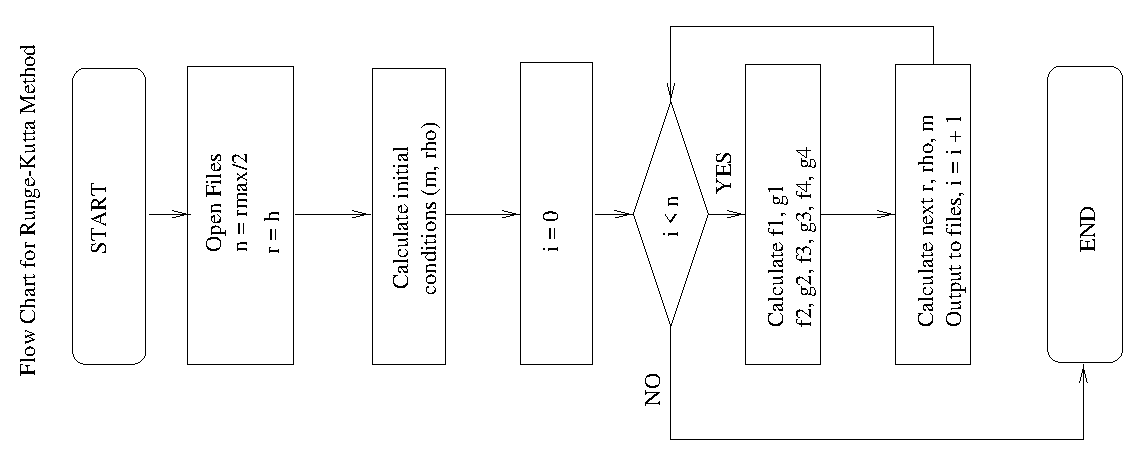
\includegraphics[width=\columnwidth,angle=-90]{figures/flow.eps}
    \end{center}
    \end{figure} 

%========================================================================

%\newpage
\section{Results}

%------------------------------------------------------------------------

    \subsection{Comparing Euler and Runge-Kutta Methods}
    Table~\ref{tbl:euler-runge-kutta} shows the values obtained for $\bar{M}$
    and $\bar{R}$ using Euler's and Runge-Kutta methods for
    a step size, $h = 0.01$ and central density $\rho_c = 10.0$.

    \begin{table}
    \caption{Comparing Euler and Runge-Kutta for $h=0.01$.} 
    \label{tbl:euler-runge-kutta} 
    \begin{center}
    \begin{tabular}{c|ccc} \hline
    $h$                 & Euler     & Runge-Kutta & Expected\\ \hline 
    $\bar{M}$           & 1.550     & 1.580       & 1.58    \\ 
    $\bar{R}$           & 1.313     & 1.298       & 1.298\\ \hline
    \end{tabular}
    \end{center}
    \end{table} 

    We can see from Table~\ref{tbl:euler-runge-kutta} 
    that the Runge-Kutta method is more accurate.

    \subsubsection{Mass Profile}
    Figures~\ref{fig:mass-euler} and~\ref{fig:mass-runge-kutta}
    show the mass profile of a white dwarf star 
    calculated using Euler's and the Runge-Kutta methods with:
    \begin{itemize}
        \item Step size $h = 0.01$
        \item $\rho_c = 10.0$
    \end{itemize}

    \begin{figure}
    \caption{Plot of $\bar{m}(\bar{r})$ using Euler's method.} 
    \label{fig:mass-euler} 
    \begin{center}
        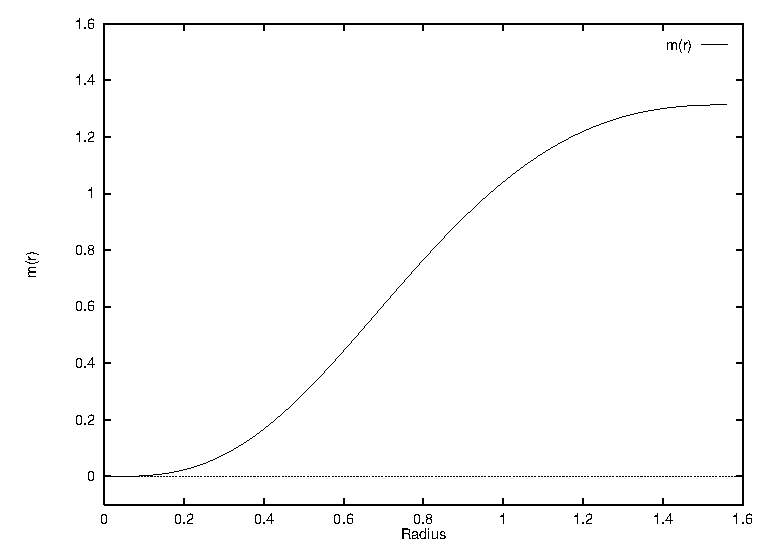
\includegraphics[width=\columnwidth]{figures/mass-euler-01}
    \end{center}
    \end{figure} 

    \begin{figure} 
    \caption{Plot of $\bar{m}(\bar{r})$ using fourth order Runge Kutta.}
    \label{fig:mass-runge-kutta}  
    \begin{center}
        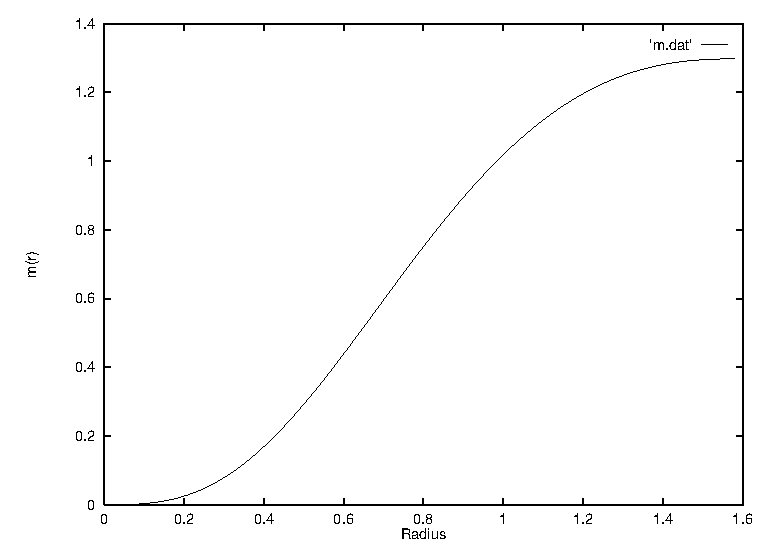
\includegraphics[width=\columnwidth]{figures/mass-rk-01}
    \end{center}
    \end{figure} 

    \subsubsection{Density Profile}
    Figures~\ref{fig:density-euler} and~\ref{fig:density-runge-kutta}
    show the density profile of a white dwarf star 
    calculated using Euler's and the Runge-Kutta methods with:
    \begin{itemize}
        \item Step size $h = 0.01$
        \item $\rho_c$ = 10.0
    \end{itemize}

    \begin{figure}
    \caption{Plot of $\bar{\rho}(\bar{r})$ using Euler's method.}
    \label{fig:density-euler} 
    \begin{center}
        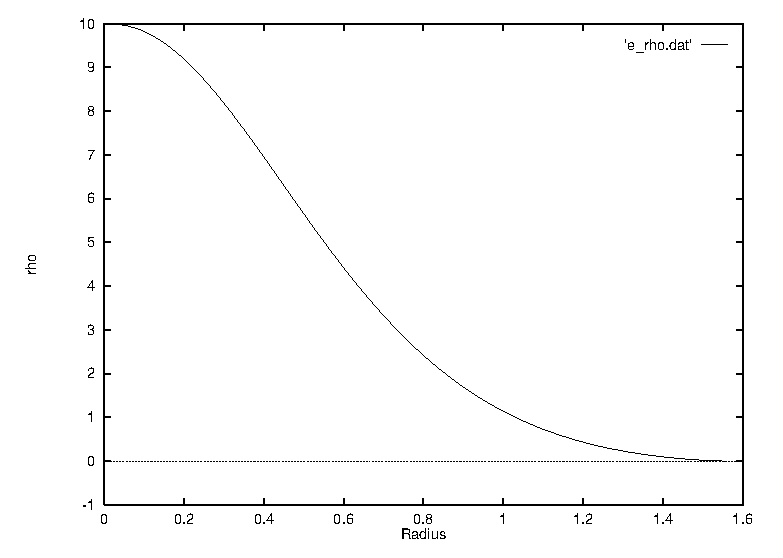
\includegraphics[width=\columnwidth]{figures/density-euler-01}
    \end{center}
    \end{figure} 

    \begin{figure} 
    \caption{Plot of $\bar{\rho}(\bar{r})$ using fourth order Runge Kutta.}
    \label{fig:density-runge-kutta} 
    \begin{center}
        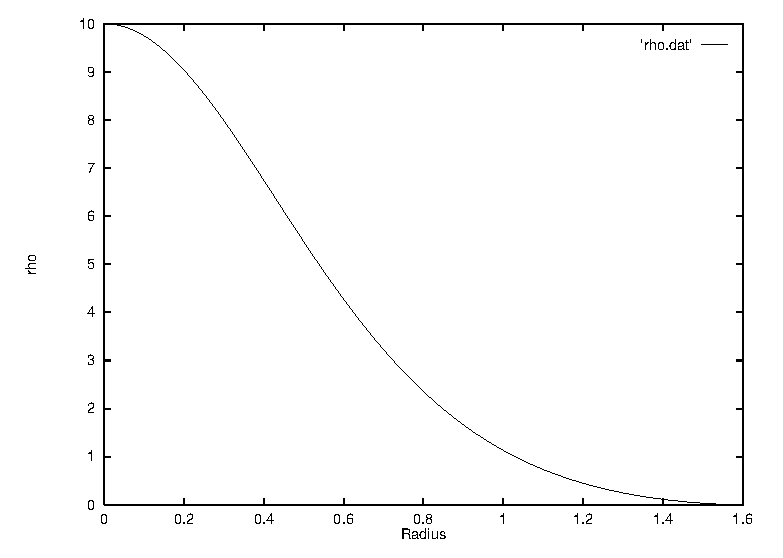
\includegraphics[width=\columnwidth]{figures/density-rk-01}
    \end{center}
    \end{figure} 

%------------------------------------------------------------------------

    \subsection{Investigating Stability with different step sizes}
    Table~\ref{tbl:R-M-euler} and~\ref{tbl:R-M-runge-kutta}
    show values of $\bar{R}$ and $\bar{M}$, with
    the central density $\rho_c = 10.0$, for different step 
    sizes $h$ using both the Euler and the Runge-Kutta methods.

    The first observation is that the Runge-Kutta algorithm reaches
    the answer faster as we increase the step size. This is to
    be expected as we know it provides more accurate results
    than the Euler algorithm.

    By looking at the column for $\bar{M}$, we see that the Runge-Kutta
    algorithm is more stable than the Euler algorithm as we decrease
    the step size.

    \begin{table}
    \caption{$\bar{R}$ and $\bar{M}$ for different values of the 
             step size $h$, using Euler's method.} 
    \label{tbl:R-M-euler}
    \begin{center}
    \begin{tabular}{r|rr} \hline
    $h$         &   $\bar{R}$   &   $\bar{M}$       \\ \hline
    0.1         &   1.3         &   1.47581763      \\ 
    0.01        &   1.55        &   1.31320078      \\ 
    0.001       &   1.587       &   1.29950998      \\ 
    0.0001      &   1.5911      &   1.29816256      \\ 
    0.00001     &   1.59157     &   1.29802791      \\ 
    0.000001    &   1.591623    &   1.29801445      \\ \hline   
    \end{tabular}
    \end{center}
    \end{table} 

    \begin{table}
    \caption{$\bar{R}$ and $\bar{M}$ for different values of the step 
             size $h$, using fourth order Runge-Kutta.}
    \label{tbl:R-M-runge-kutta} 
    \begin{center}
    \begin{tabular}{r|rr} \hline
    $h$         &   $\bar{R}$   &   $\bar{M}$       \\ \hline
    0.1         &   1.5         &   1.29518167      \\ 
    0.01        &   1.58        &   1.29799616      \\ 
    0.001       &   1.591       &   1.29801293      \\ 
    0.0001      &   1.5916      &   1.29801295      \\ 
    0.00001     &   1.59162     &   1.29801295      \\ 
    0.000001    &   1.591629    &   1.29801295      \\ \hline
    \end{tabular}
    \end{center}
    \end{table} 

    \subsection{Investigation of mass and density at large central densities}
    Figure~\ref{fig:mass-profiles} and~\ref{fig:density-profiles} 
    plot the mass and density profiles for
    the white dwarf star for a range of values of the central density $\rho_c$,
    (with $Y_e = 1$), using the fourth order Runge-Kutta algorithm with
    a step size of $h = 0.01$.
    These plots are the solutions for $\bar{\rho}(\bar{r})$ and $\bar{m}(\bar{r})$,
    of~\ref{eq:density} and~\ref{eq:mass}.

    Using the solutions to the differential equations we determine 
    $\bar{R}$ and $\bar{M}$ for the different values of $\rho_c$.
    These results are shown in Table~\ref{tbl:central-density}. 

    \begin{table}
    \caption{$\bar{R}$ and $\bar{M}$ for $h = 0.01$ at different
              values of the central density $\rho_c$.} 
    \label{tbl:central-density} 
    \begin{center}
    \begin{tabular}{r|rr} \hline
    $\rho_c$&   $\bar{R}$   &   $\bar{M}$       \\ \hline
    0.1     &   2.57        &   0.22178884     \\ 
    1       &   2.49        &   0.70706357     \\ 
    10      &   1.58        &   1.29799616     \\ 
    100     &   0.95        &   1.73552752      \\ 
    1000    &   0.53        &   1.93285505      \\ 
    10000   &   0.27        &   1.99681784      \\ 
    100000  &   0.13        &   2.01300131      \\ 
    1000000 &   0.05        &   1.76970419      \\ \hline
    \end{tabular}
    \end{center}
    \end{table} 

    As the central density increases, the mass of the star increases.
    As the central density increases the radius decreases because there 
    is more mass and hence the star is falling in on itself yet there still
    exists the equilibrium between the gravitational force and the electron
    degeneracy pressure. However, a smaller radius increases the gravitational
    field of the star, since we know from Newton's law of gravitation
    the gravitational force proportional to $1/r^2$.

    \begin{equation}
        F_g = -\frac{GmM}{r^2}
    \end{equation}

    Therefore, the greater the mass and the smaller the radius of the 
    star the greater the gravitational force of the star, pushing the star
    in on itself. 

    For extremely high values of the central density, the resulting radius
    and mass may by be so high it results in an extremely large gravitational
    field which is too strong for it to stay in equilibrium and hence 
    the assumptions made about equations~\ref{eq:density} and~\ref{eq:mass}
    no longer hold and the star will collapse in on itself. Then depending on
    the mass of the star it may become a neutron star, or if the mass is 
    extremely large, a black hole.

    Figure~\ref{fig:mass-profiles} shows the computed mass profiles for different values of 
    $\rho_c$ and Figure~\ref{fig:density-profiles} shows the computed density profiles
    for different values of $\rho_c$. 

    %\subsubsection{Mass profiles for different values of $\rho_c$}

    \begin{figure*} 
    \caption{Mass profiles for different values of $\rho_c$} 
    \label{fig:mass-profiles} 
    \begin{center}
    \begin{tabular}{p{7cm}p{7cm}}  
        $\rho_c = 0.1$ \newline 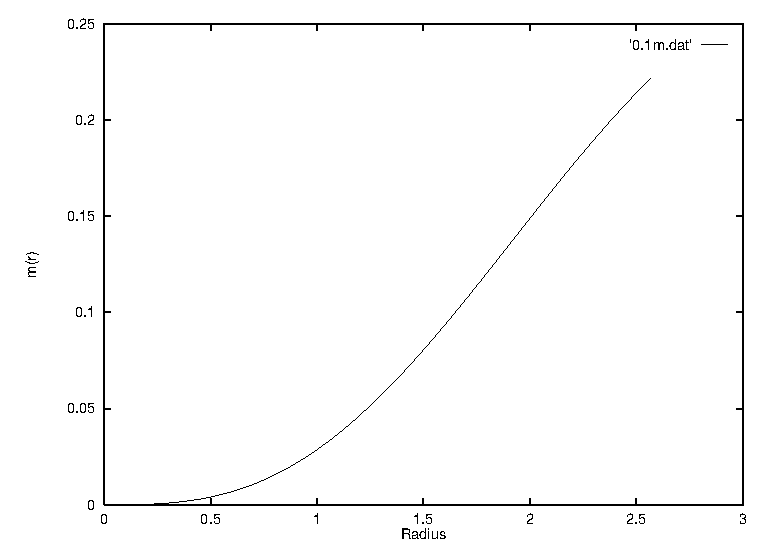
\includegraphics[width=7cm]{figures/0-1m.eps} & 
        $\rho_c = 1.0$ \newline 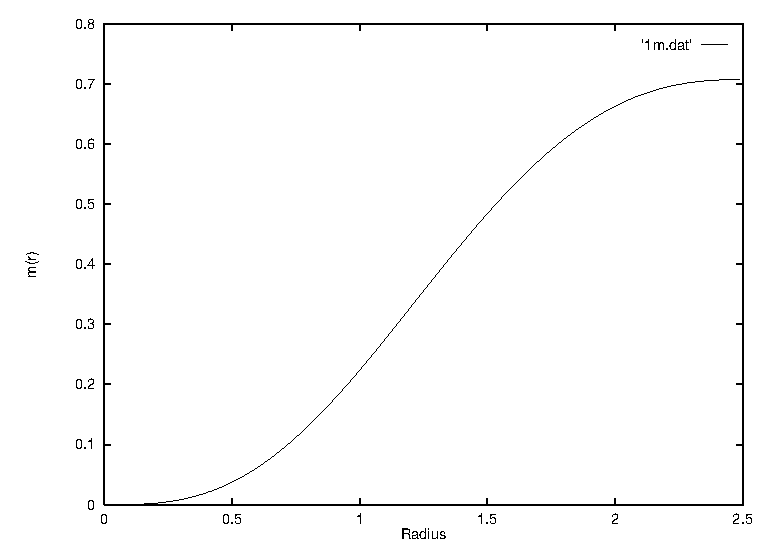
\includegraphics[width=7cm]{figures/1m.eps}  
        \\
        $\rho_c = 10.0$ \newline 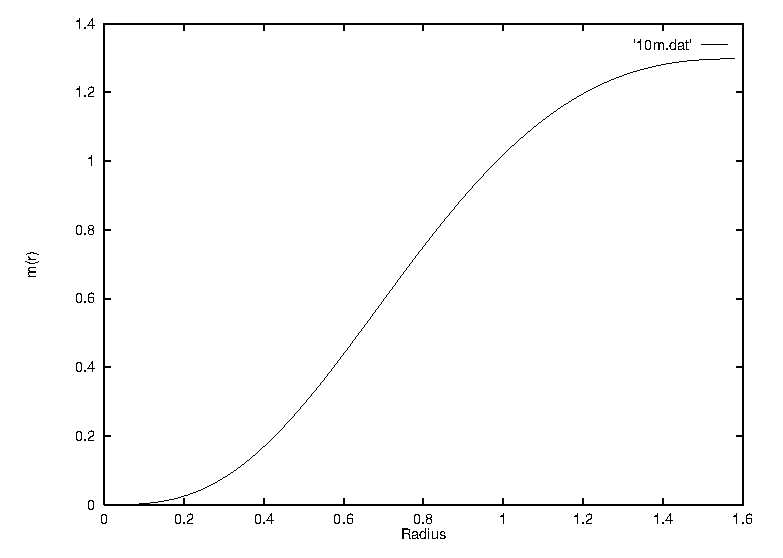
\includegraphics[width=7cm]{figures/10m.eps}  & 
        $\rho_c = 10^2$ \newline 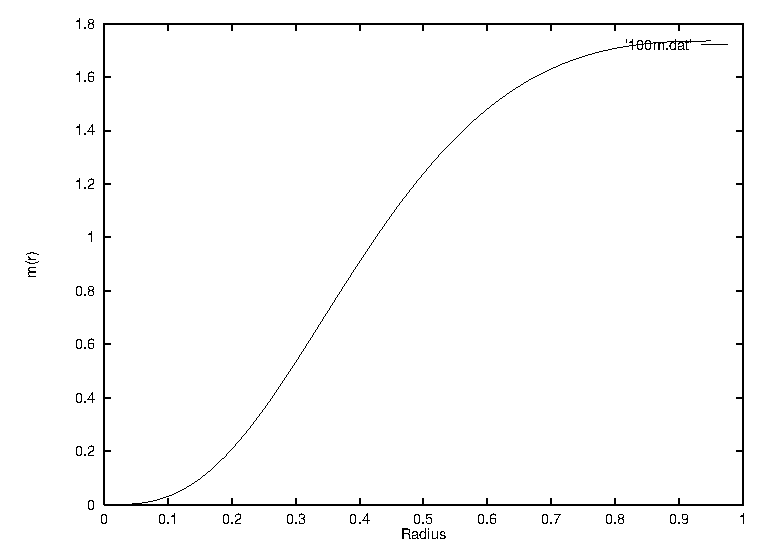
\includegraphics[width=7cm]{figures/100m.eps}    
        \\
        $\rho_c = 10^3$ \newline 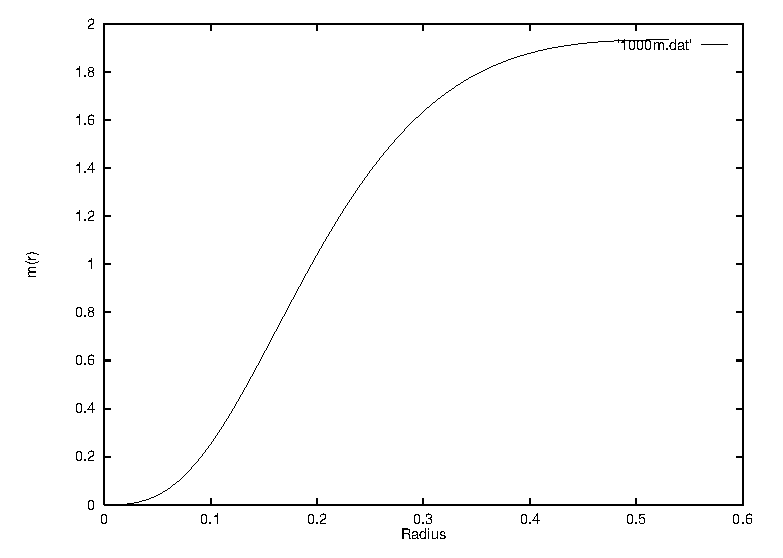
\includegraphics[width=7cm]{figures/1000m.eps}  & 
        $\rho_c = 10^4$ \newline 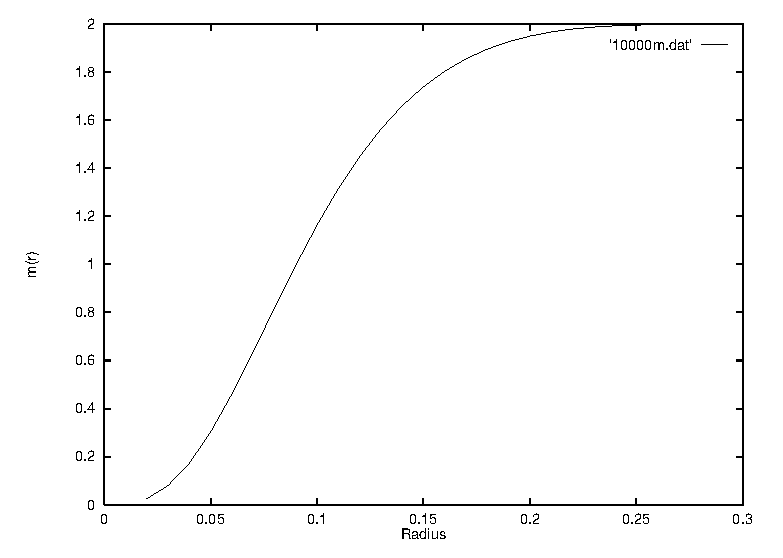
\includegraphics[width=7cm]{figures/10000m.eps}   
        \\
        $\rho_c = 10^5$ \newline 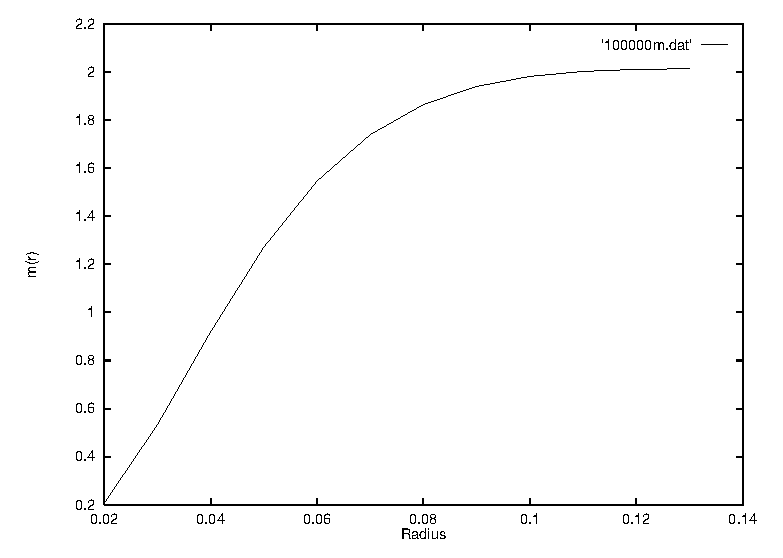
\includegraphics[width=7cm]{figures/100000m.eps}  & 
        $\rho_c = 10^6$ \newline 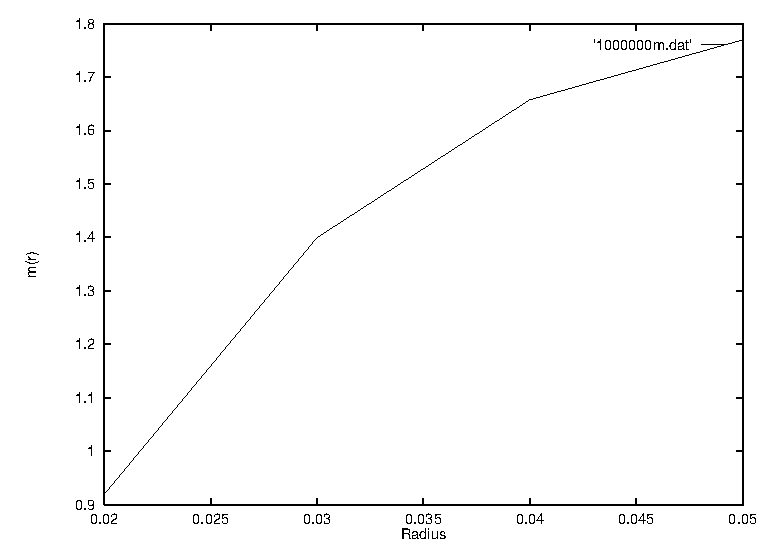
\includegraphics[width=7cm]{figures/1000000m.eps}
        \\ 
    \end{tabular}
    \end{center}
    \end{figure*} 

    %\subsubsection{Density profiles for different values of $\rho_c$}

    \begin{figure*} 
    \caption{Density profiles for different values of $\rho_c$} 
    \label{fig:density-profiles} 
    \begin{center}
    \begin{tabular}{p{7cm}p{7cm}}  
        $\rho_c = 0.1$ \newline 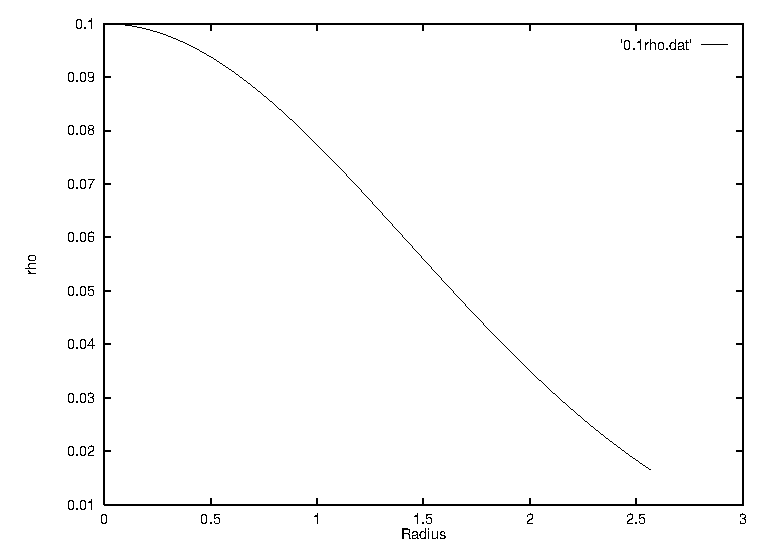
\includegraphics[width=7cm]{figures/0-1rho.eps} & 
        $\rho_c = 1.0$ \newline 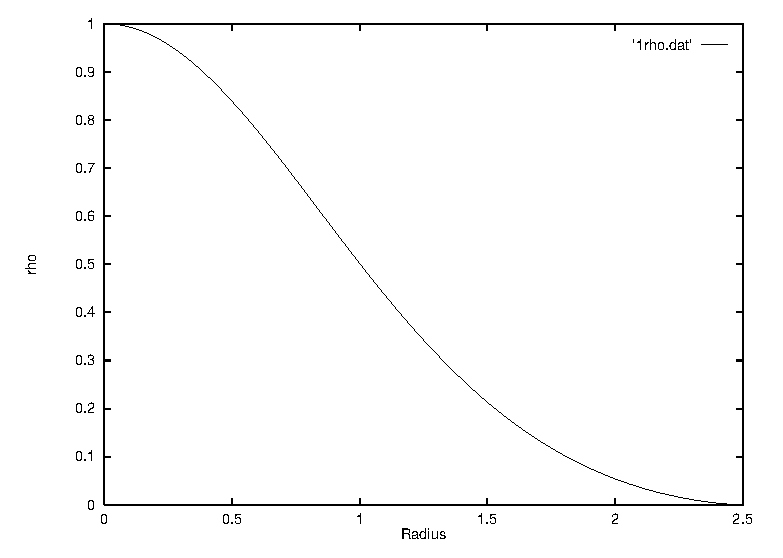
\includegraphics[width=7cm]{figures/1rho.eps}  
        \\
        $\rho_c = 10.0$ \newline 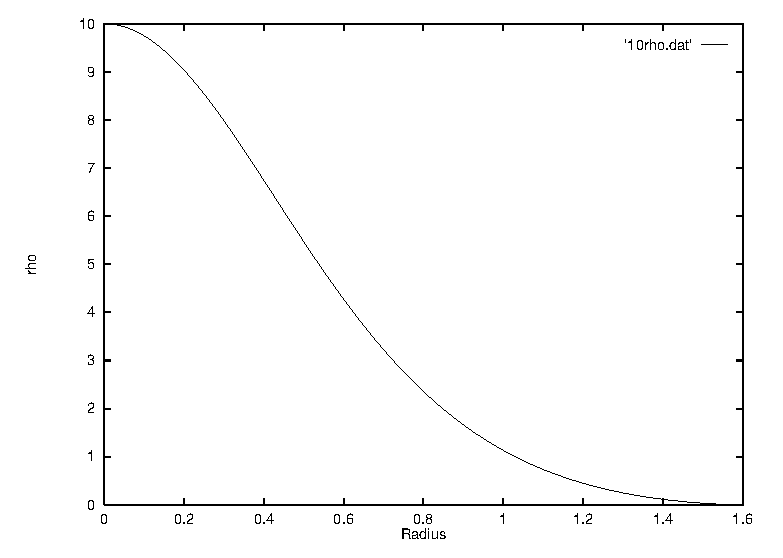
\includegraphics[width=7cm]{figures/10rho.eps}  & 
        $\rho_c = 10^2$ \newline 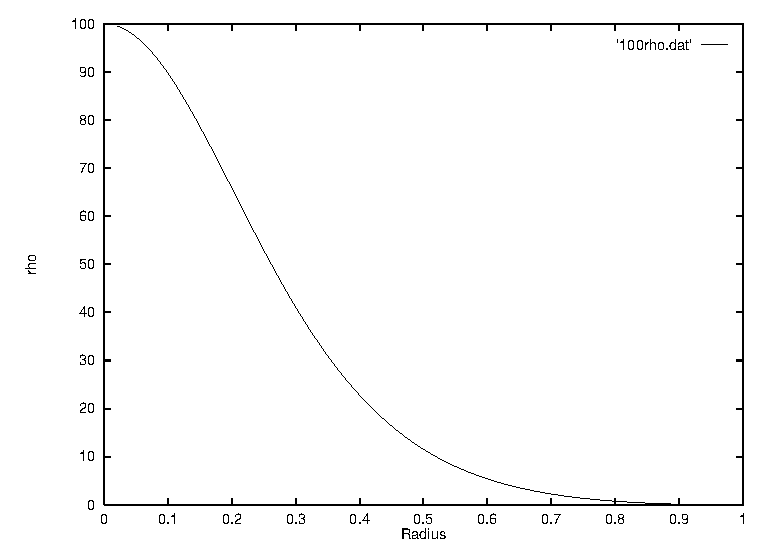
\includegraphics[width=7cm]{figures/100rho.eps}    
        \\
        $\rho_c = 10^3$ \newline 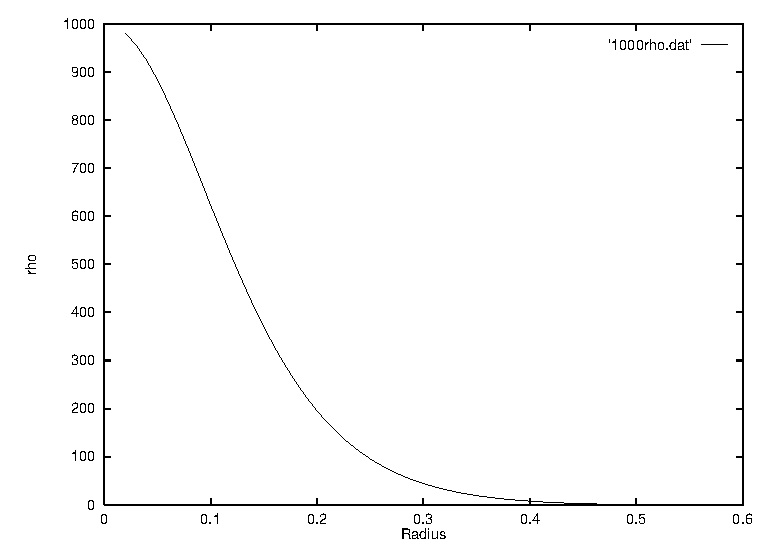
\includegraphics[width=7cm]{figures/1000rho.eps}  & 
        $\rho_c = 10^4$ \newline 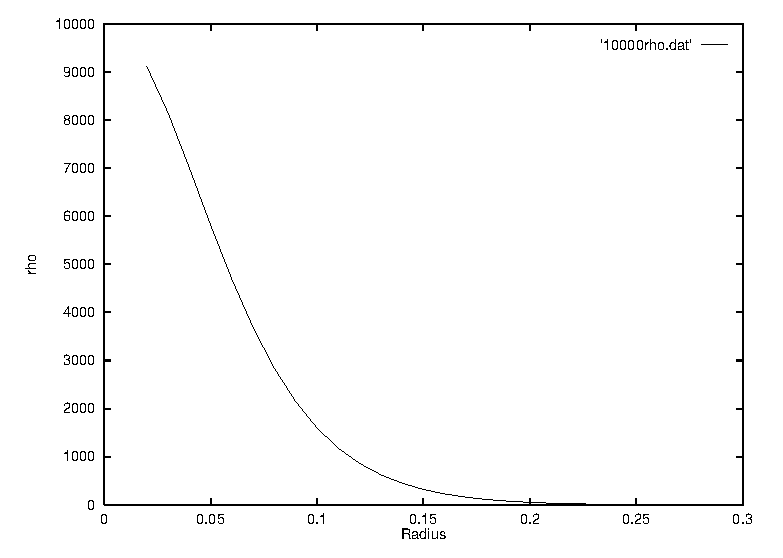
\includegraphics[width=7cm]{figures/10000rho.eps}   
        \\
        $\rho_c = 10^5$ \newline 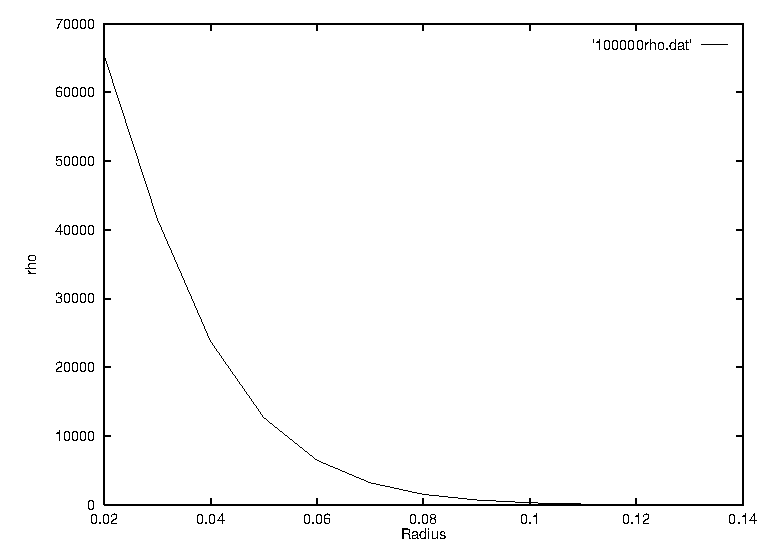
\includegraphics[width=7cm]{figures/100000rho.eps}  & 
        $\rho_c = 10^6$ \newline 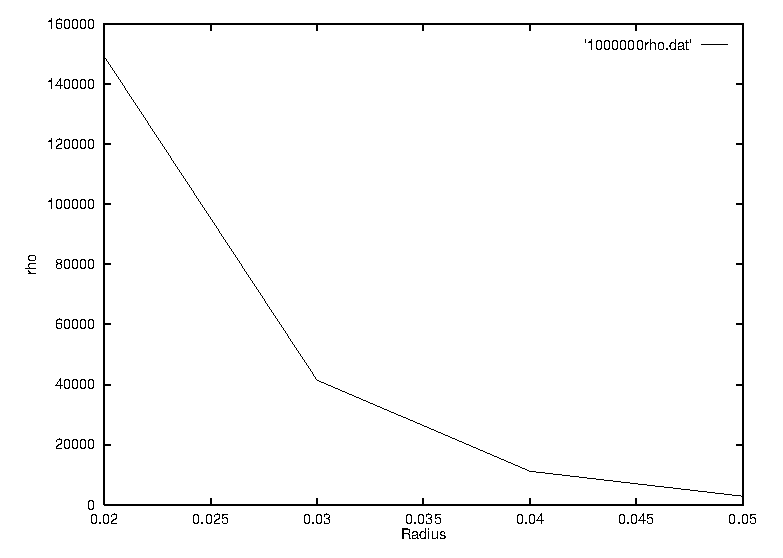
\includegraphics[width=7cm]{figures/1000000rho.eps}
        \\ 
    \end{tabular}
    \end{center}
    \end{figure*} 

    \section{Calculations for Sirius B and 40 Eri B} 

    For values of $Y_e \not= 1$, we have:
    \[ M(Y_e) = Y_{e}^2 \frac{M_0}{M_{sun}} \bar{M}(Y_e = 1)\]
    \[ R(Y_e) = Y_e \frac{R_0}{R_{sun}} \bar{R}(Y_e = 1)\]
    Using values from Koonin~[1] we can calculate:

    \[ \frac{M_0}{M_{sun}} = 
        \frac{5.67 \times 10^{33} Y_e^2 gm}{1.98 \times 10^{33} gm} =  2.863636 Y_e^2\]

    \[ \frac{R_0}{R_{sun}} = 
        \frac{7.72 \times 10^8 Y_e cm}{6.95 \times 10^{10} cm} = 1.11079 \times 10^{-2} Y_e\]

    \subsection{Sirius B} 
    
    \begin{itemize} 
        \item $M = 1.053 \pm 0.028$ 
        \item $R = 0.0074 \pm 0.0006$ 
    \end{itemize} 
    
    Table~\ref{tbl:results-sirius-b} shows the results for the radius $R$, for the program 
    running for a number of different central densities. Here $R$ is:

    \[ R = Y_e \frac{R_0}{R_{sun}} \bar{R}(Y_e = 1) \]

    \begin{table} 
        \caption{Results for Sirius B} 
        \label{tbl:results-sirius-b} 
        \begin{center}
        \begin{tabular}{r|crr} \hline
        $\rho_c$    &   $\bar{R}(Y_e=1)$   & R ($Y_e = 0.5)$ & R ($Y_e = 0.464$)\\ \hline
        10.0        &   1.58        & 0.00877525071    & 0.00814343218   \\
        15.0        &   1.45        & 0.00877525071    & 0.00814343218   \\ 
        16.0        &   1.45        & 0.00805323641    & 0.00747340295 \\
        18.0        &   1.40        & 0.00777553860    & 0.00721569940\\ 
        20.0        &   1.37        & 0.00760891992    & 0.00706107727   \\ 
        22.0        &   1.34        & 0.00744230123    & 0.00690645514  \\ \hline
        \end{tabular}
        \end{center}
    \end{table} 

    We see from Table~\ref{tbl:results-sirius-b} that the central density of Sirius B is:
    \begin{itemize}
        \item $\rho_c = 22.0$ (Solar Units) for $Y_e = 0.5$ (Carbon)
        \item $\rho_c = 16.0$ (Solar Units) for $Y_e = 0.464$ (Iron)
    \end{itemize}

    We see that these results are within error. Sirius B has a mass very similar
    to that of the Sun but a much smaller radius. This implies that the density
    of Sirius B is greater than the Sun, resulting in a smaller radius.
    What this means is that the atoms which make up Sirius B are likely to
    be heavier than those in the Sun. We are more likely to find greater
    amounts of heavy nuclei such as Carbon and Iron.
    Without knowing the exact proportions of Carbon and Iron in Sirius B,
    we can only estimate the the central density of this what dwarf is
    somewhere in the range $16.0 \leq \rho_c \leq 22.0$ in solar units.

    \subsection{40 Eri B}

    \begin{itemize} 
        \item $M = 0.48 \pm 0.02 $
        \item $R = 0.0124 \pm 0.0005 $
    \end{itemize}

    Table~\ref{tbl:results-40-eri-b} shows the results for $R$, with the program running
    with different values of the central density.

    \begin{table}
        \caption{Results for 40 Eri B} 
        \label{tbl:results-40-eri-b} 
        \begin{center}
            \begin{tabular}{r|crr} \hline
            $\rho_c$    &   $\bar{R}(Y_e=1)$   & R ($Y_e = 0.5)$   & R ($Y_e = 0.464$)\\ \hline
            1.0         &   2.49        & 0.0138293508      & 0.0128336368 \\
            1.2         &   2.41        & 0.0133850343      & 0.0124213111 \\
            1.5         &   2.31        & 0.0128296387      & 0.0119059040 \\
            1.7         &   2.25        & 0.0124964013      & 0.0115966597 \\
            2.0         &   2.19        & 0.0121631640       & 0.0112874155 \\
            3.0         &   2.02        & 0.0112189914      & 0.0104112234 \\
            5.0         &   1.83        & 0.0101637397      & 0.0094319499 \\
            6.0         &   1.76        & 0.0097749628     & 0.0090711649 \\ \hline
            \end{tabular}
        \end{center}
    \end{table} 

    We see from Table~\ref{tbl:results-40-eri-b} that the central density of 40 Eri B is:
    \begin{itemize}
        \item $\rho_c = 1.7$ (Solar Units) for $Y_e = 0.5$ (Carbon)
        \item $\rho_c = 1.2$ (Solar Units) for $Y_e = 0.464$ (Iron)
    \end{itemize}

    We see that 40 Eri B has mass that is is approximately half that of
    the Sun, and a radius only 1\% that of the Sun's. However we see that
    the central density of 40 Eri B is in the range $1.2 \leq \rho_c \leq 1.7$
    in solar units. If a star half the like the Sun where to have it's radius 
    reduced to 1\% of it's original size, it's density would increase
    dramatically because:
        \[ \rho = \frac{M}{V} = \frac{M}{\frac{4}{3} \pi r^3} \]
    This suggests that that the atoms in 40 Eri B are lighter than those
    found in the Sun. It is likely that 40 Eri B consists almost totally
    of Hydrogen and Helium, with only traces of heavier nuclei.

    \section{References}
        \begin{enumerate}
            \item \emph{Computational Physics}, Koonin and Meredith
        \end{enumerate} 


%========================================================================

    \onecolumn
    \appendix[Code Listing: star.f]
    \showcode{src/star.f} 

\end{document}

%========================================================================

